\chapter{Instrumental learning}


Form of control learning that aims to learn action-outcome associations:
\begin{itemize}
    \item When a reinforcer is likely to occur.
    \item Which actions bring to those reinforcers.
\end{itemize}
This allows the animal to act in anticipation of a reinforcer.

Depending on the outcome, the effect varies:
\begin{descriptionlist}
    \item[Positive reinforcement] \marginnote{Positive reinforcement}
        Delivering an appetitive outcome to an action increases the probability of emitting it.

    \item[Positive punishment] \marginnote{Positive punishment}
        Delivering an aversive outcome to an action decreases the probability of emitting it.
    
    \item[Negative reinforcement] \marginnote{Negative reinforcement}
        Omitting an aversive outcome to an action increases the probability of emitting it.
    
    \item[Negative punishment] \marginnote{Negative punishment}
        Omitting an appetitive outcome to an action decreases the probability of emitting it.
\end{descriptionlist}

\begin{table}[H]
    \centering
    \begin{tabular}{r|cc}
        \toprule
                            & \textbf{Delivery}                         & \textbf{Omission} \\
        \midrule
        \textbf{Appetitive} & Positive reinforcement (\texttt{+prob})   & Negative punishment (\texttt{-prob}) \\
        \textbf{Aversive}   & Positive punishment (\texttt{-prob})      & Negative reinforcement (\texttt{+prob}) \\
        \bottomrule
    \end{tabular}
    \caption{Summary of the possible effects}
\end{table}



\section{Types of schedule}

There are two types of learning:
\begin{descriptionlist}
    \item[Continuous schedule] \marginnote{Continuous schedule}
        The desired action is followed by the outcome every time.
        \begin{remark}
            More effective to teach a new association.
        \end{remark}

    \item[Partial schedule] \marginnote{Partial schedule}
        The desired action is not always followed by the outcome.
        \begin{remark}
            Learning is slower but the response is more resistant to extinction.
        \end{remark}

        There are four types of partial schedules:
        \begin{descriptionlist}
            \item[Fixed-ratio] 
                Outcome available after a specific number of responses.

                This results in a high and steady rate of response, with a brief pause after the outcome is delivered.


            \item[Variable-ratio] 
                Outcome available after an unpredictable number of responses.

                This results in a high and steady rate of response.


            \item[Fixed-interval] 
                Outcome available after a specific interval of time.

                This results in a high rate of response near the end of the interval and a slowdown after the outcome is delivered.


            \item[Variable-interval] 
                Outcome available after an unpredictable interval of time.

                This results in a slow and steady rate of response.
        \end{descriptionlist}
\end{descriptionlist}

\begin{minipage}{0.55\linewidth}
    \begin{example}[Aplysia Californica]
        An Aplysia Californica will withdraw its gill upon stimulating the siphon.
        \begin{itemize}
            \item Repeated mild stimulations will induce a habituation of the reflex.
            \item Repeated intense stimulations will induce a sensitization of the reflex.
        \end{itemize}
    \end{example}
\end{minipage}
\begin{minipage}{0.4\linewidth}
    \centering
    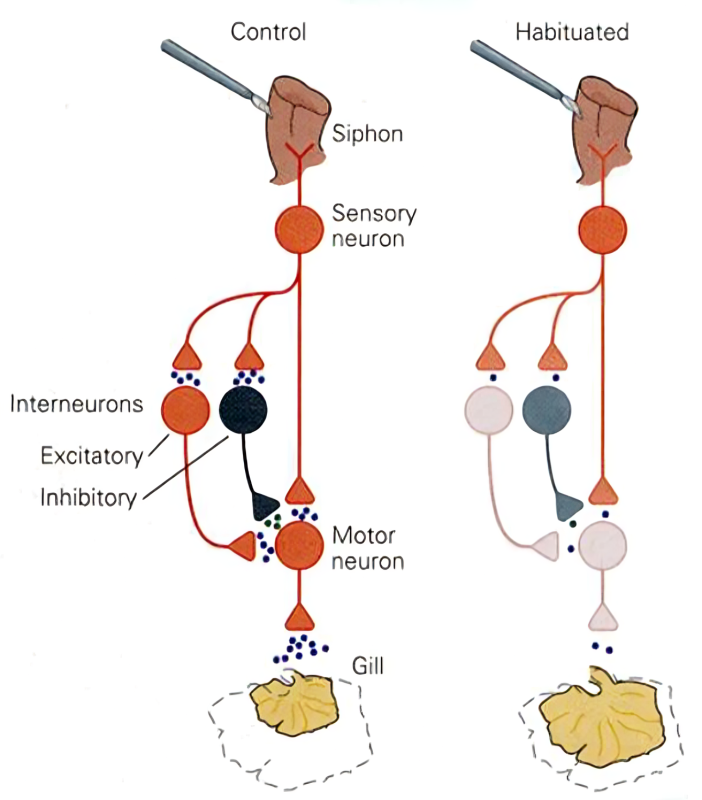
\includegraphics[width=0.9\linewidth]{./img/gill_habituation.png}
\end{minipage}



\section{Dopamine}

There is evidence that dopamine is involved in learning action-outcome associations.

\begin{description}
    \item[Striatal activity on unexpected events] \marginnote{Striatal activity on unexpected events}
        When an unexpected event happens, there is a change in the activity of the striatum.
        There is an increase in response when the feedback is positive and a decrease when negative.

        \begin{@empty}
            \small
            \begin{example}[Microelectrodes in substantia nigra]
                The activity of the substantia nigra of patients with Parkinson's disease is measured during a probabilistic instrumental learning task.
                The task consists of repeatedly drawing a card from two decks, followed by positive or negative feedback depending on the deck.

                \begin{figure}[H]
                    \centering
                    \begin{subfigure}{0.25\linewidth}
                        \centering
                        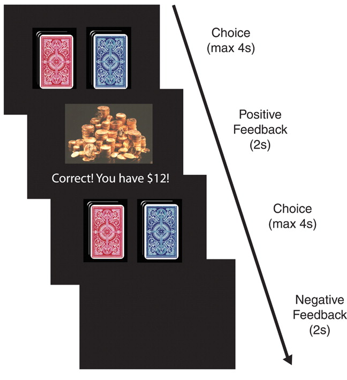
\includegraphics[width=\linewidth]{./img/instrumental_dopamine_sn1.png}
                    \end{subfigure}
                    \begin{subfigure}{0.55\linewidth}
                        \centering
                        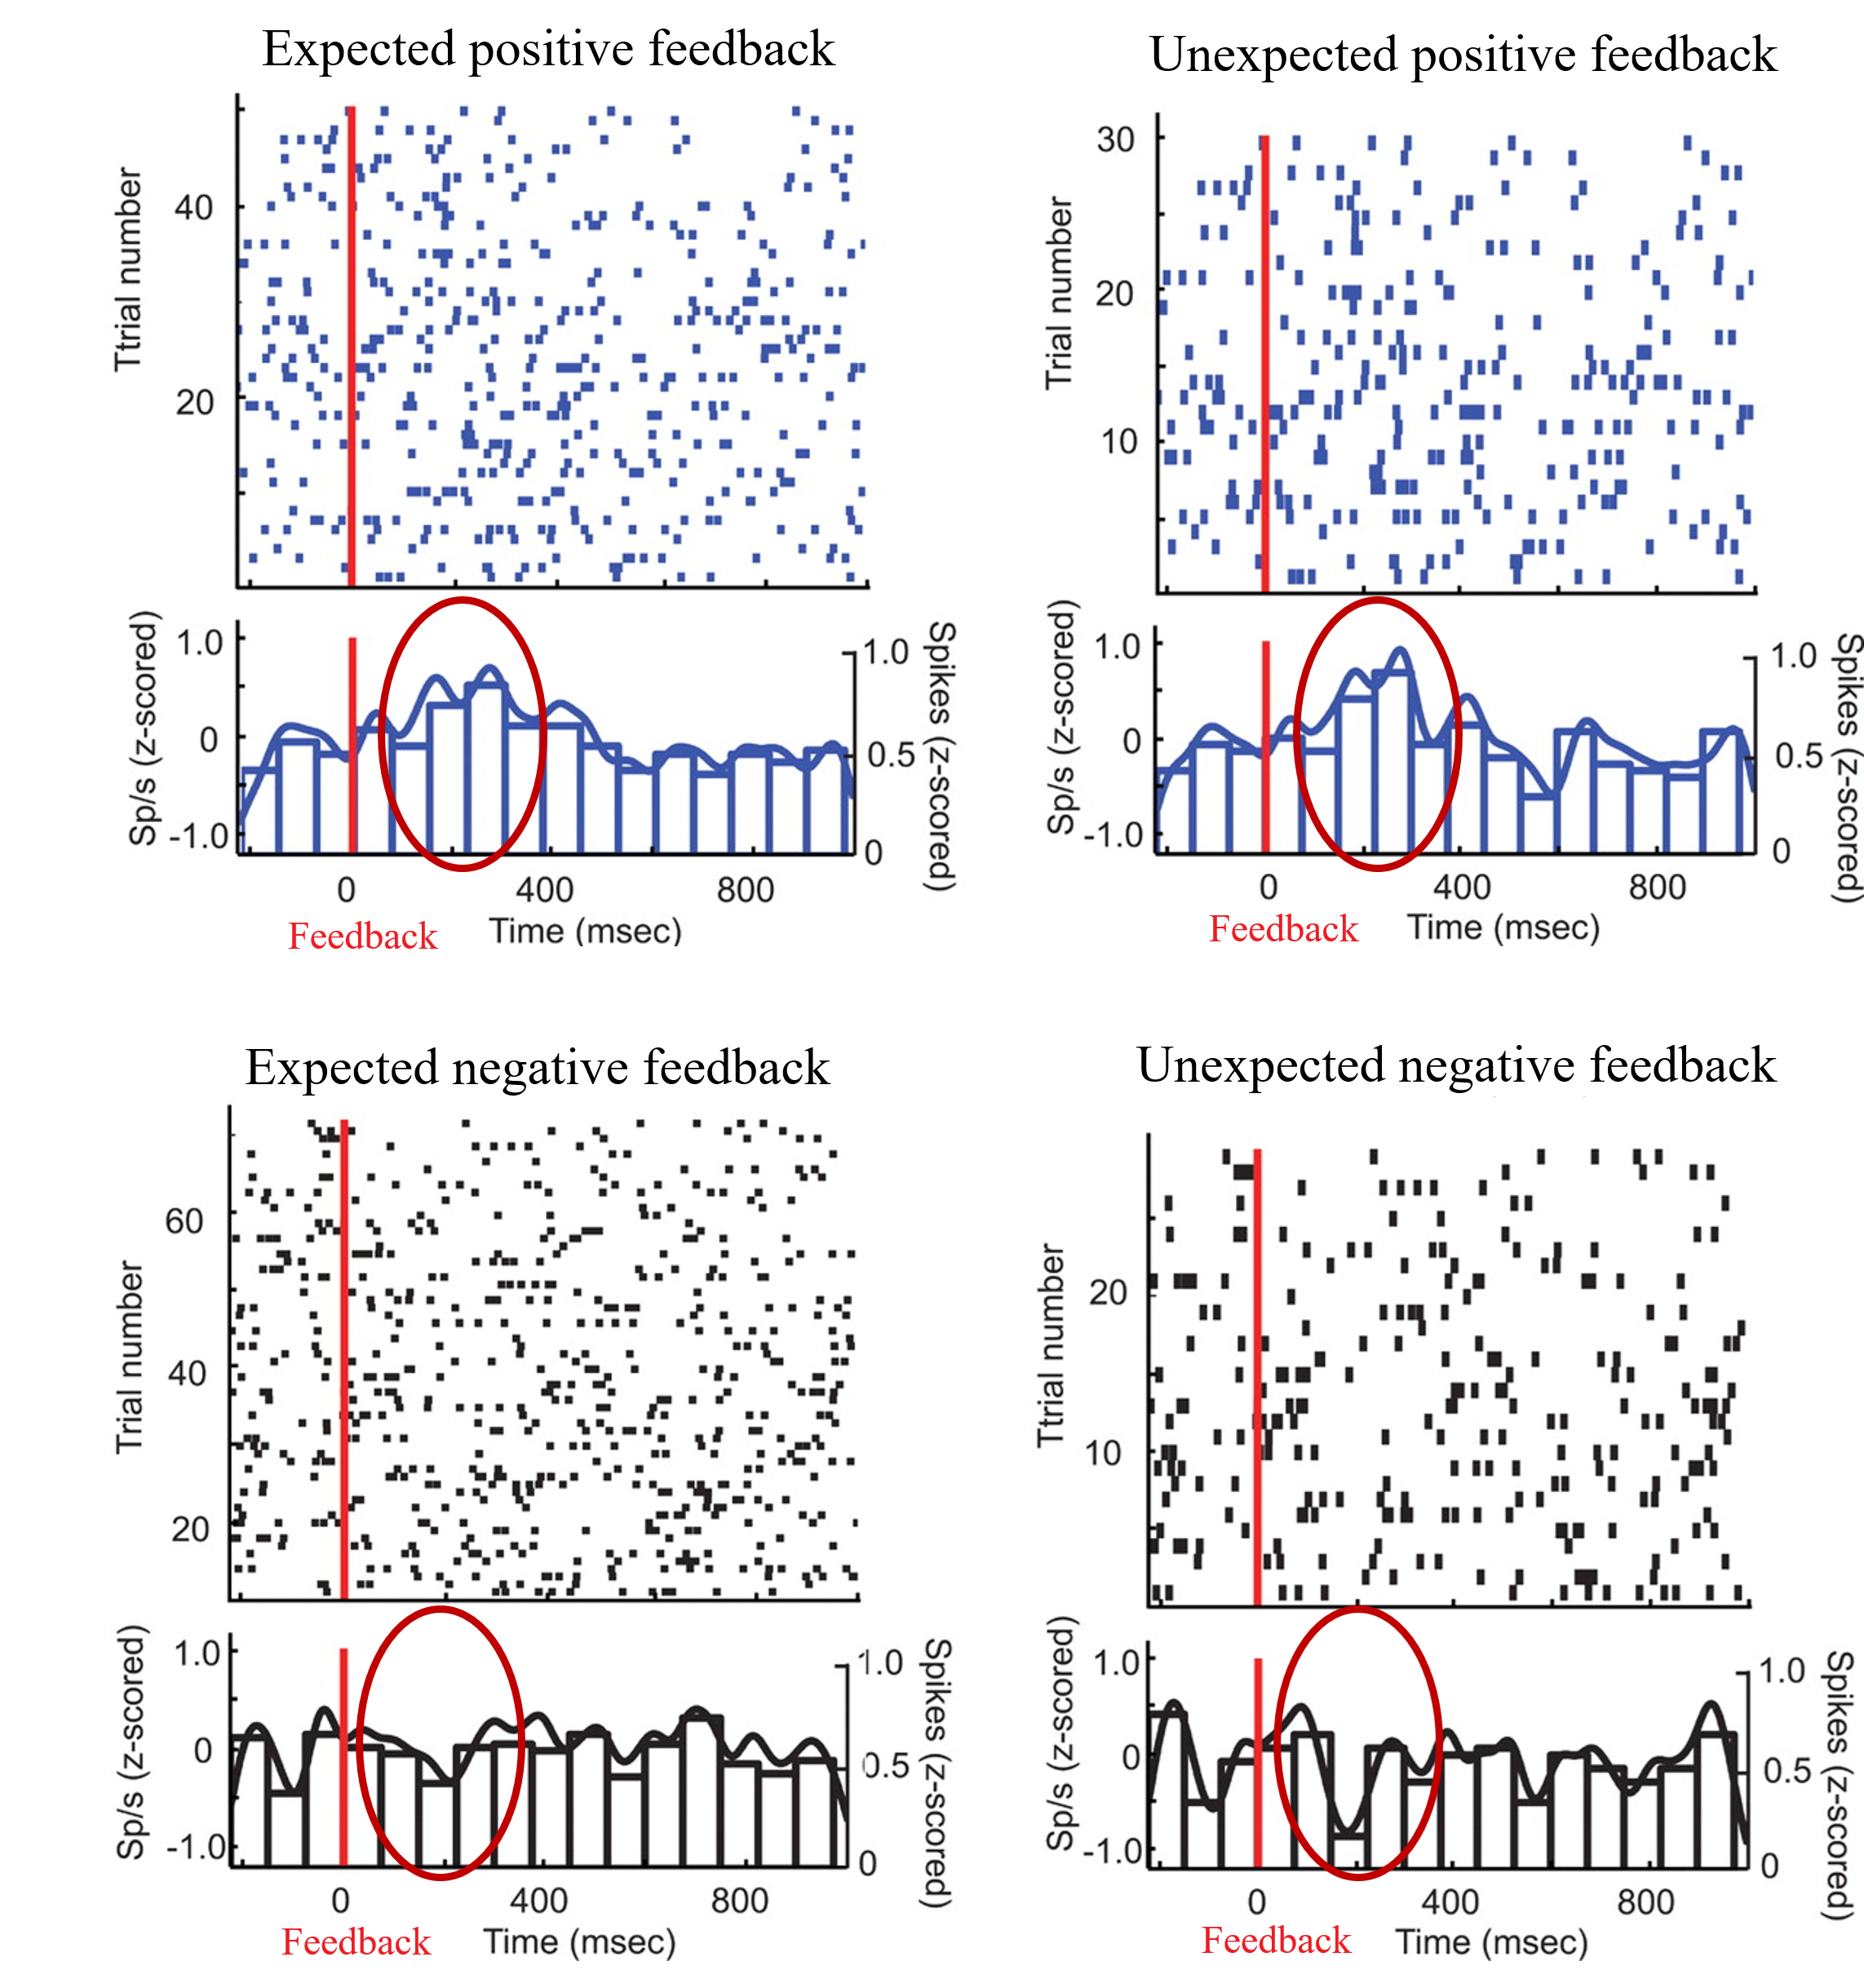
\includegraphics[width=\linewidth]{./img/instrumental_dopamine_sn2.png}
                    \end{subfigure}
                \end{figure}

                The increase and decrease in striatal activity can be clearly seen when the feedback is unexpected.
            \end{example}
        \end{@empty}

    \item[Dopamine effect on behavior] \marginnote{Dopamine effect on behavior}
        The amount of dopamine changes the learning behavior:
        \begin{itemize}
            \item Low levels of dopamine cause an impairment in learning from positive feedback.
                This happens because positive prediction errors cannot occur.
            
            \item High levels of dopamine cause an impairment in learning from negative feedback.
                This happens because negative prediction errors cannot occur.
        \end{itemize}

        \begin{@empty}
            \small
            \begin{example}[Probabilistic selection task]
                This instrumental learning task has two phases:
                \begin{descriptionlist}
                    \item[Learning]
                        There are three pairs of stimuli (symbols) and, at each trial, a pair is presented to the participant who selects one.
                        For each pair, a symbol has a higher probability of providing positive feedback while the other is more likely to be negative.
                        Moreover, the probabilities are different among the three pairs.

                        \begin{center}
                            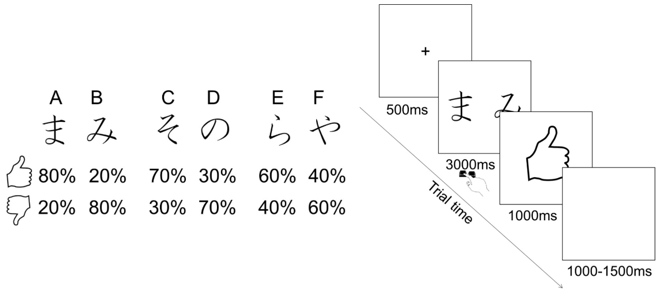
\includegraphics[width=0.55\linewidth]{./img/instrumental_dopamine_selection1.png}
                        \end{center}

                        Participants are required to learn by trial and error the stimulus in each pair that leads to a positive reward.
                        Note that learning could be accomplished by:
                        \begin{itemize}
                            \item Recognizing the more rewarding stimulus.
                            \item Recognizing the less rewarding stimulus.
                            \item Both.
                        \end{itemize}

                    \item[Testing]
                        Aims to assess if participants learned to select positive feedback or avoid negative feedback.

                        The same task as above is repeated but all combinations of the stimuli among the three pairs are possible.
                \end{descriptionlist}

                Three groups of participants are considered for this experiment:
                \begin{enumerate}
                    \item Those who took the cabergoline drug (dopamine antagonist).
                    \item Those who took the haloperidol drug (dopamine agonist).
                    \item Those who took a drug without effects (placebo).
                \end{enumerate}

                \begin{center}
                    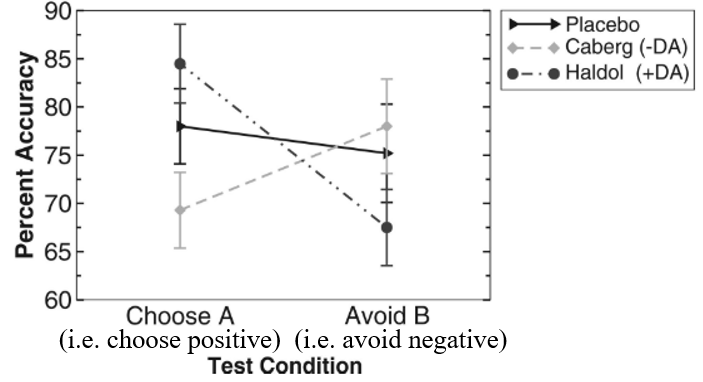
\includegraphics[width=0.55\linewidth]{./img/instrumental_dopamine_selection2.png}
                \end{center}

                Results show that:
                \begin{enumerate}
                    \item Cabergoline inhibited positive feedback learning.
                    \item Haloperidol enhanced positive feedback learning.
                    \item Placebo learned positive and negative feedback equally.
                \end{enumerate}
            \end{example}
        \end{@empty}
        
        \begin{@empty}
            \small
            \begin{example}
                It has been observed that:
                \begin{itemize}
                    \item Reward prediction errors are correlated with activity in the left posterior putamen and left ventral striatum.
                    \item Punishment prediction errors are correlated with activity in the right anterior insula.
                \end{itemize}

                \begin{center}
                    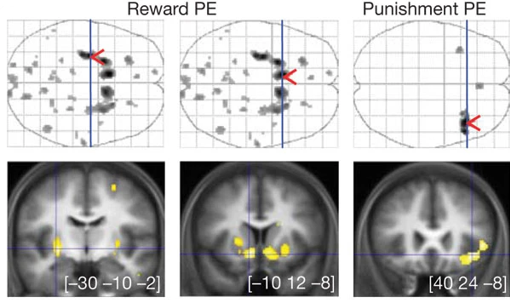
\includegraphics[width=0.5\linewidth]{./img/pe_location.png}
                \end{center}
            \end{example}
        \end{@empty}

    \item[Actor-critic model] \marginnote{Actor-critic model}
        Model to correlate Pavlovian and instrumental learning. 
        It is composed by:
        \begin{itemize}
            \item The cortex is responsible for representing the current state.
            \item The basal ganglia implement two computational models:
                \begin{descriptionlist}
                    \item[Critic] \marginnote{Critic}
                        Learns stimulus-outcome associations and is active in both Pavlovian and instrumental learning.
                        It might be implemented in the ventral striatum, the amygdala and the orbitofrontal cortex.
                
                    \item[Actor] \marginnote{Actor}
                        Learns stimulus-action associations and is only active during instrumental learning.
                        It might be implemented in the dorsal striatum.
                \end{descriptionlist}
        \end{itemize}
\end{description}

\begin{@empty}
    \small
    \begin{example}[Food and cocaine]
        \phantom{}
        \begin{itemize}
            \item Food-induced dopamine response is modulated by the reward expectations that promote learning until the prediction matches the actual outcome.
            \item Cocaine-induced dopamine response causes a continuous increase in the predicted reward that
                will eventually surpass all other cues and bias decision-making towards cocaine.
        \end{itemize}
        \begin{center}
            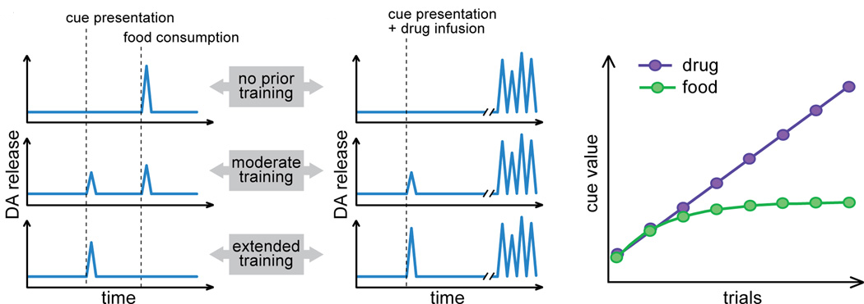
\includegraphics[width=0.7\linewidth]{./img/dopamine_food_cocaine.png}
        \end{center}
    \end{example}
\end{@empty}